\documentclass[a4paper, 12pt]{article}%тип документа

%отступы
\usepackage[left=2cm,right=2cm,top=2cm,bottom=3cm,bindingoffset=0cm]{geometry}

%Русский язык
\usepackage[T2A]{fontenc} %кодировка
\usepackage[utf8]{inputenc} %кодировка исходного кода

%Вставка картинок
\usepackage{wrapfig}
\usepackage{graphicx}
\graphicspath{{pictures/}}
\DeclareGraphicsExtensions{.pdf,.png,.jpg}

%Графики
\usepackage{multirow}
\usepackage{pgfplots}
\pgfplotsset{compat=1.9}

%Математика
\usepackage{amsmath, amsfonts, amssymb, amsthm, mathtools}

%Заголовок
\author{Hasib Sifat \\
Faculty of Physical and Quantum Electronics \\
GROUP Б04-105}
\title{\textbf{LABORATORY WORK 3.4.2 \\ 
Curie-Weiss Law}}
\begin{document}
\maketitle

\begin{abstract}
In this paper I've shown the experimental result of the temperature dependence of the magnetic susceptibility of a ferromagnet above the Curie point and found the Curie point of Gadolinium with $81.05\%$ accuracy.
\end{abstract}
\section{Theoretical Description} Substances with non-zero atomic magnetic moments have paramagnetic properties. The external magnetic field orients the magnetic moments, which in the absence of the field were located in space in a chaotic manner. However, at $T\rightarrow 0$, thermal motion less and less prevents the magnetic moments of atoms from being oriented in one direction with an arbitrarily weak external field. In ferromagnets - under the influence of exchange forces - this happens when the temperature drops not to absolute zero, but to the Curie temperature $\Theta$. As the temperature $T$ rises, the disorienting effect of the thermal motion of particles increases, and the magnetic susceptibility of ferromagnets decreases according to the Curie-Weiss law


\begin{equation}
		\label{eq:Kuri-Veicca}
		\chi \propto \frac{1}{T-\Theta_p},
	\end{equation}
where $\Theta_p$ is a temperature close to the Curie temperature, since at $T\approx\Theta$ the formula~(\ref{eq:Kuri-Veicca}) is not accurate enough. At $T < \Theta_p$, the sample has ferromagnetic properties and can retain magnetization, at $T > \Theta_p$, the sample behaves like a paramagnetic for which the relationship between $B$ and $H$ is unambiguous: $I = \chi H$, $B = \mu H$. Gadolinium was chosen for the study, since its Curie point lies in the range of room temperatures.


\section{Experimental Setup}
The scheme of the installation for checking the Curie-Weiss law is shown in Fig.~\ref{rus:ustanovka}. The investigated ferromagnetic sample (gadolinium) is located inside a hollow self-induction coil, which serves as the inductance of the oscillatory circuit, which is part of the LC-autogenerator. The autogenerator is assembled on a KP-103 field-effect transistor and mounted as a separate unit.
\begin{figure}
		\center{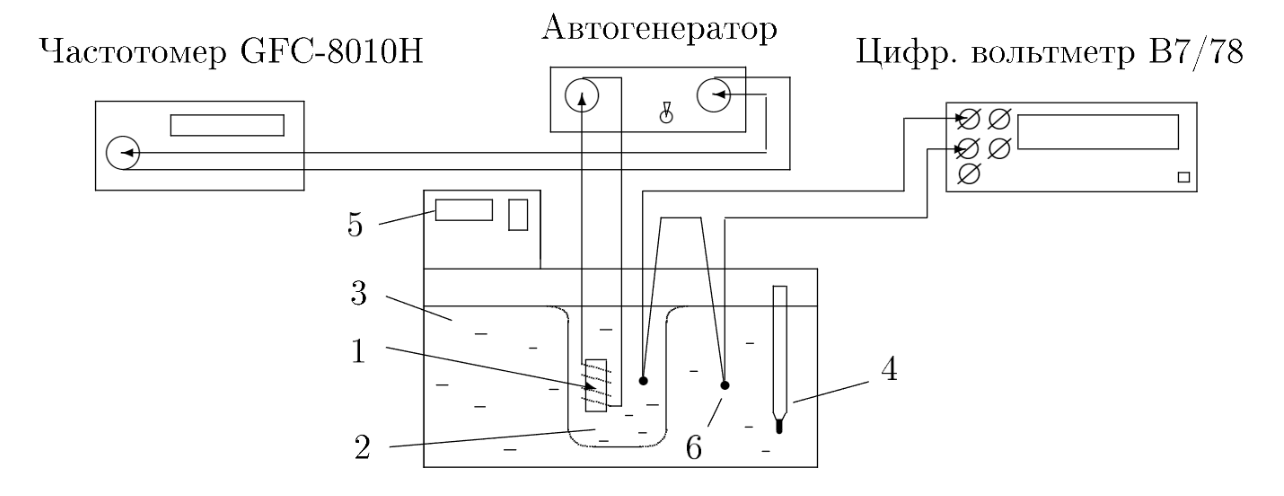
\includegraphics[scale=0.5]{Fig1.png}}
		\caption{Experimental Scheme}
		\label{ris:ustanovka}
\end{figure}
	
To understand the exact experimental setup, I add the original experimental setup. 
\begin{figure}
		\center{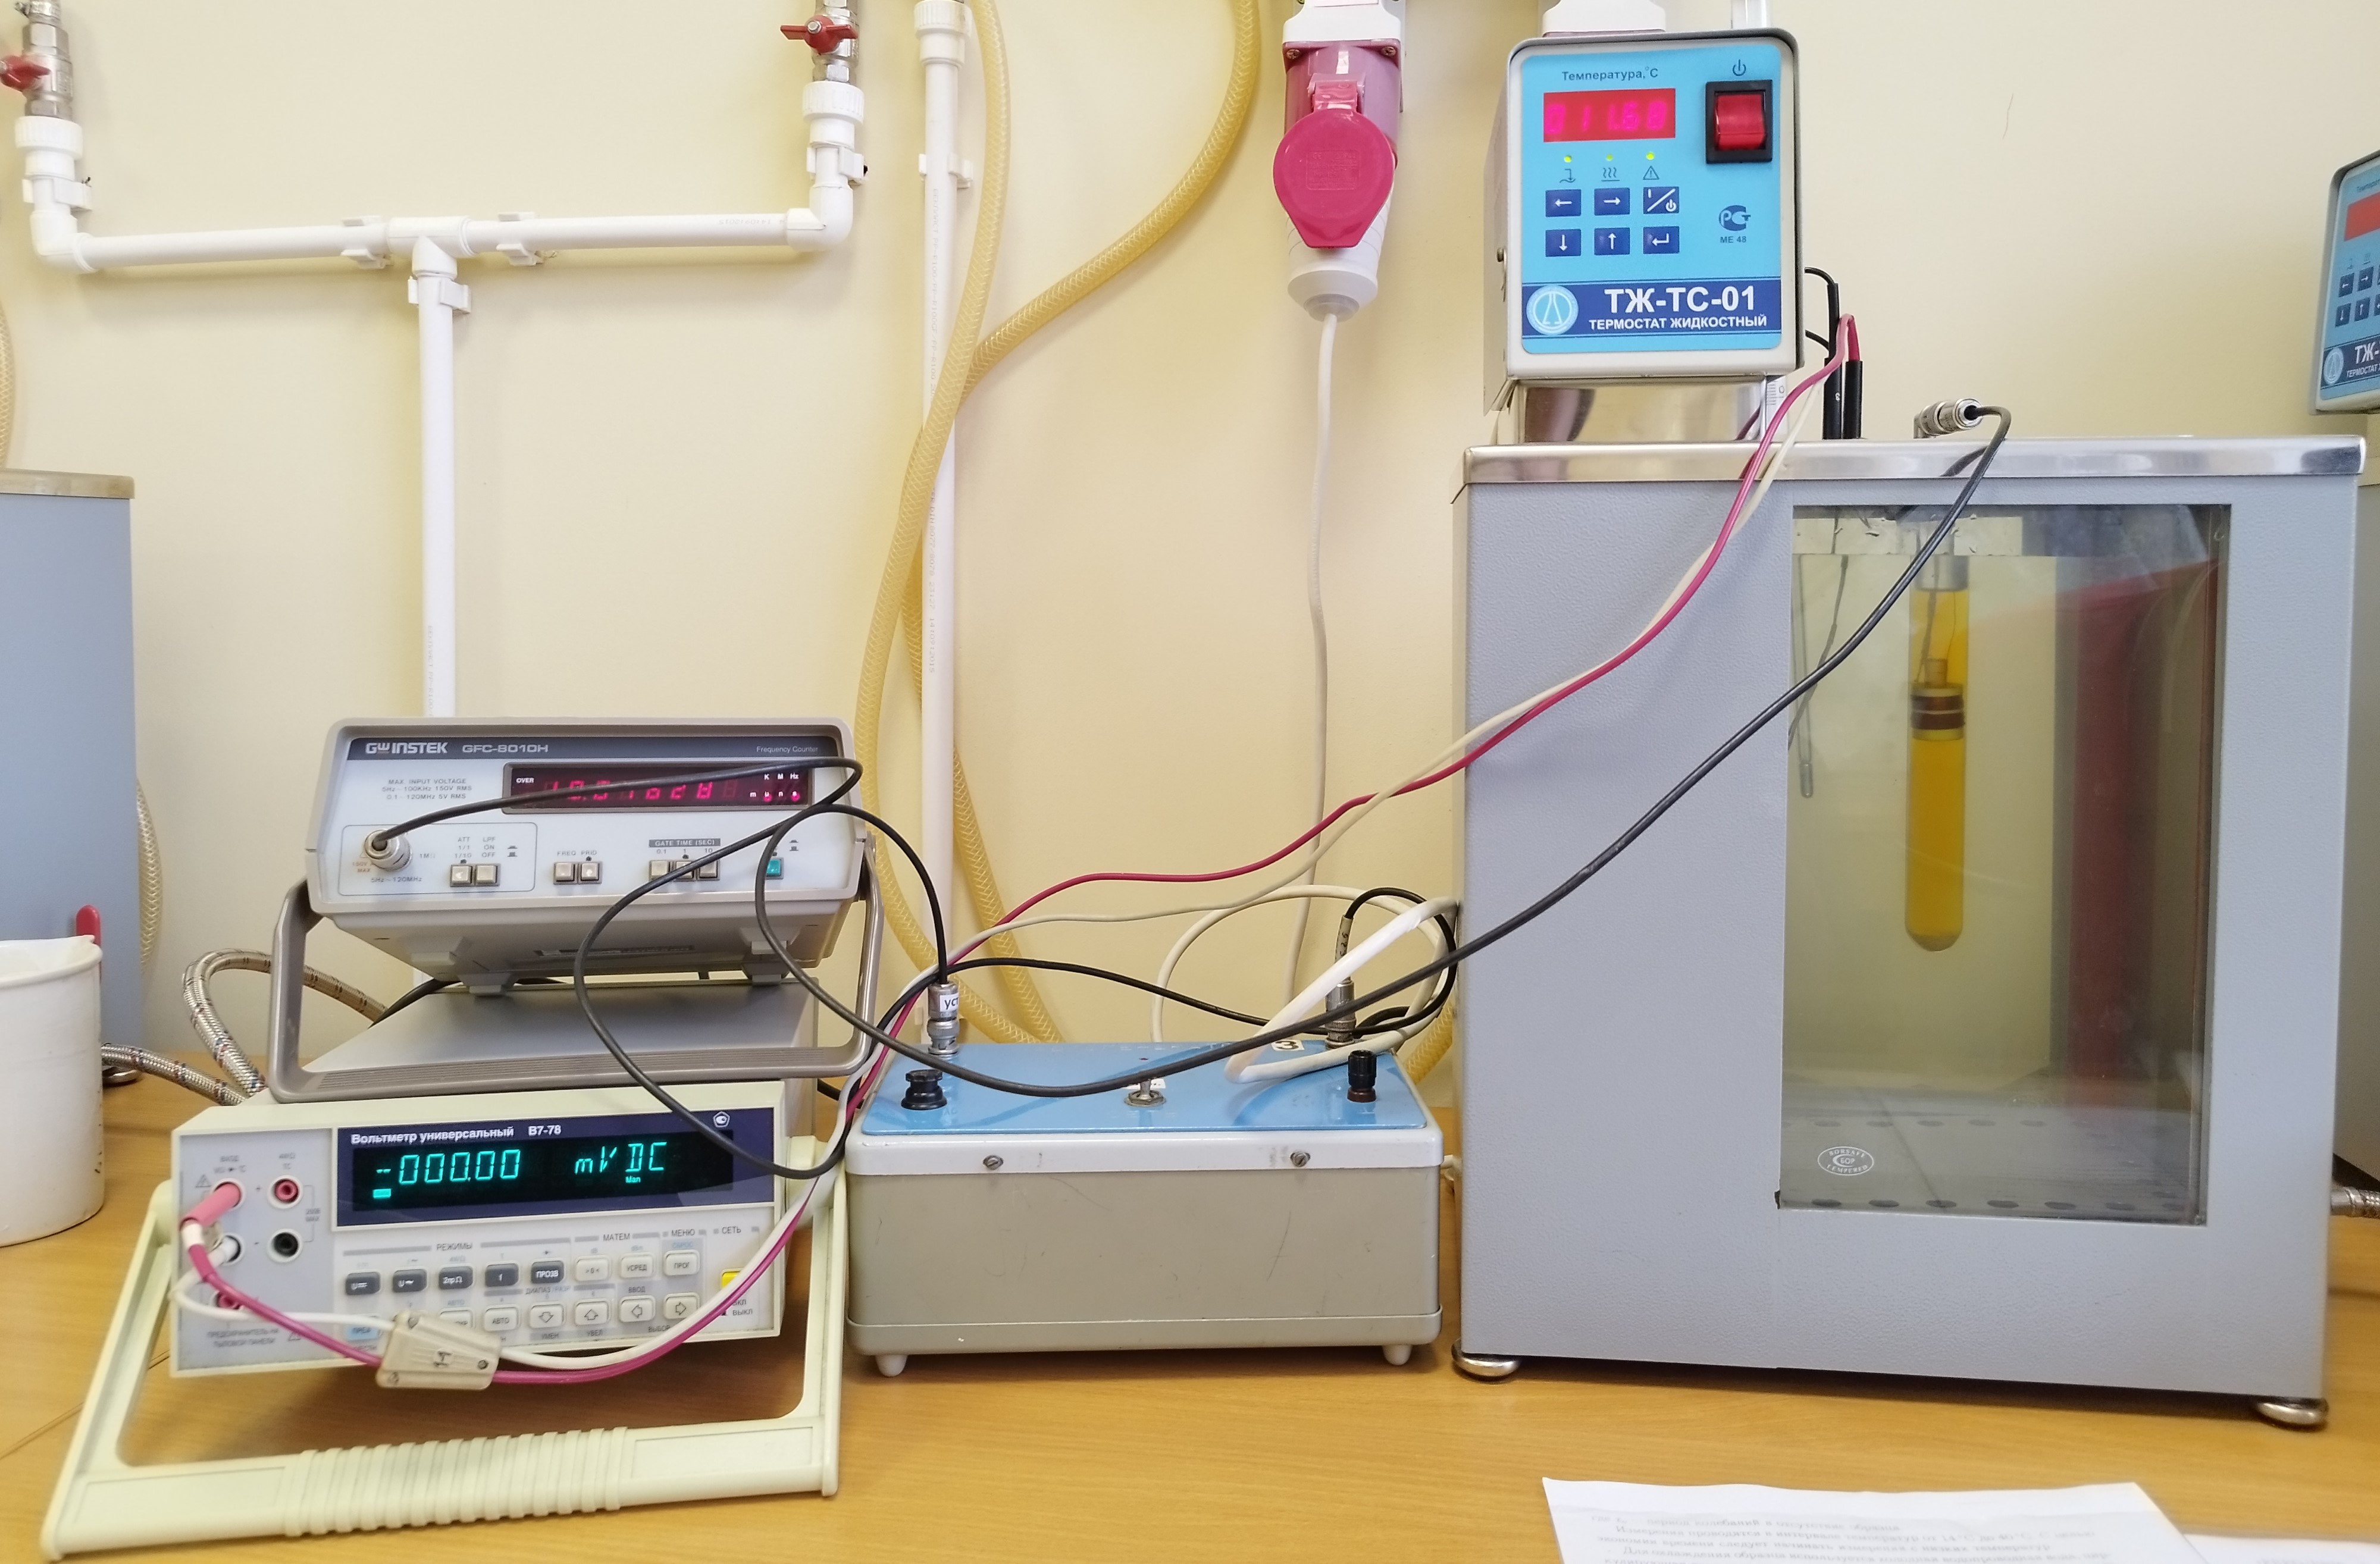
\includegraphics[scale=0.1]{Fig2.jpg}}
		\caption{Real Experimental Installation}
		\label{ris:ustanovka}
\end{figure} 
	
The magnetic susceptibility of the sample $\chi$ is determined by the change in the self-induction of the coil. Denoting by $L$ the self-induction of a coil with a sample and by $L_0$ its self-induction in the absence of a sample, we obtain
\begin{equation*}
		(L-L_0)\propto \chi.
	\end{equation*}

When the self-induction of the sample changes, the oscillation period of the self-oscillator changes:
\begin{equation*}
		\tau = 2\pi \sqrt{LC},
\end{equation*}
where $C$ is the capacitance of the oscillator circuit. The period of oscillation in the absence of the sample is determined by the self-induction of the empty coil:
\begin{equation*}
		\tau_0 = 2\pi \sqrt{L_0C}.
\end{equation*}

So, the Curie-Weiss law is valid if the relation is fulfilled:
\begin{equation}
		\frac{1}{\chi} \propto (T-\Theta_p) \propto \frac{1}{\tau^2-\tau_0^2}
\end{equation}

where $\tau_{o}$ is the oscillation period in the absence of a sample. Measurements are carried out in the temperature range from $12^{\circ}\mathrm{C}$ to $40^{\circ}\mathrm{C}.$ In order to save time, measurements should be started at low temperatures. To cool the sample, cold tap water is used, circulating around a vessel with a working fluid (distilled water); the working fluid is constantly mixed. The value of the stabilized temperature is set on the display 5 of the thermostat. An internal electric heater, not shown in the figure, is used for heating.\\
\newline
When the temperature of the working fluid in the vessel approaches the set temperature, the continuous operation of the heater automatically switches to a pulse mode (the heater turns on and off) - the temperature stabilization process begins. The temperature of the test sample is always slightly different from the temperature of distilled water in the vessel. After the water has reached Set temperature, there is a slow process of temperature equalization sample and water. Their temperature difference is controlled using a copper-constantane thermocouple 6 and a digital voltmeter. One of the thermocouple junctions is in thermal contact with the sample, and the other is immersed in water. The ends of the thermocouple are connected to a digital voltmeter. It is recommended to measure the oscillation period of the autogenerator at the moment when the specified temperature difference becomes $\leqslant 0.5^{\circ}\mathrm{C} .$ Thermocouple sensitivity $\mathrm{K}=24$ deg$/ \mathrm{mV}$
\section{Experimental Data}

Let's measure the dependence of $\tau$ from the temperature of the sample and enter the results in the table below: Remember for finding $T_0$ we will use $T_0 = T_m + \Delta UK$ where $T_m$ is measurement temperature. The given $\tau_0 = 9.045$


\begin{table}
\begin{center}
\begin{tabular}{|l|l|l|l|l|}
\hline
$\tau$, $\mu$s                          & $U$, mV                          & $T_{m}^{\circ} \mathrm{C}$      & $1 / (\tau^2 - \tau_0^2)$      & $T_0^{\circ} \mathrm{C}$      \\ \hline
10.9894                              & -0.0116                          & 14.10            & 0.0256                         & 13.82       \\ \hline
10.7851                              & -0.0170                          & 16.02            & 0.0289                         & 15.61       \\ \hline
10.5752                              & -0.0189                          & 18.01            & 0.0333                         & 17.56       \\ \hline
10.3338                              & -0.0191                          & 20.01            & 0.0400                         & 19.55       \\ \hline
9.9411                               & -0.0147                          & 22.05             & 0.0588                         & 21.69       \\ \hline
9.6091                               & -0.0175                          & 24.02            & 0.0950                         & 23.60       \\ \hline
9.4281                               & -0.0136                          & 26.04            & 0.1413                         & 25.71       \\ \hline
9.3489                               & -0.0147                          & 28.03            & 0.1789                         & 27.68       \\ \hline
9.2974                               & -0.0164                          & 30.03            & 0.2159                         & 29.64       \\ \hline
9.2601                               & -0.0151                            & 32.04            & 0.2539                         & 31.68       \\ \hline
9.2338                               & -0.0150                            & 34.04            & 0.2897                         & 33.68       \\ \hline
9.2143                               & -0.0158                            & 36.03            & 0.3234                         & 35.65       \\ \hline
9.1991                               & -0.0159                            & 38.03             & 0.3556                         & 37.65       \\ \hline
9.1876                               & -0.0175                            & 40.02             & 0.3846                         & 39.60       \\ \hline
\end{tabular}
    \caption{Measurement Data}
    \label{data}
\end{center}
\end{table}



\begin{figure}
		\center{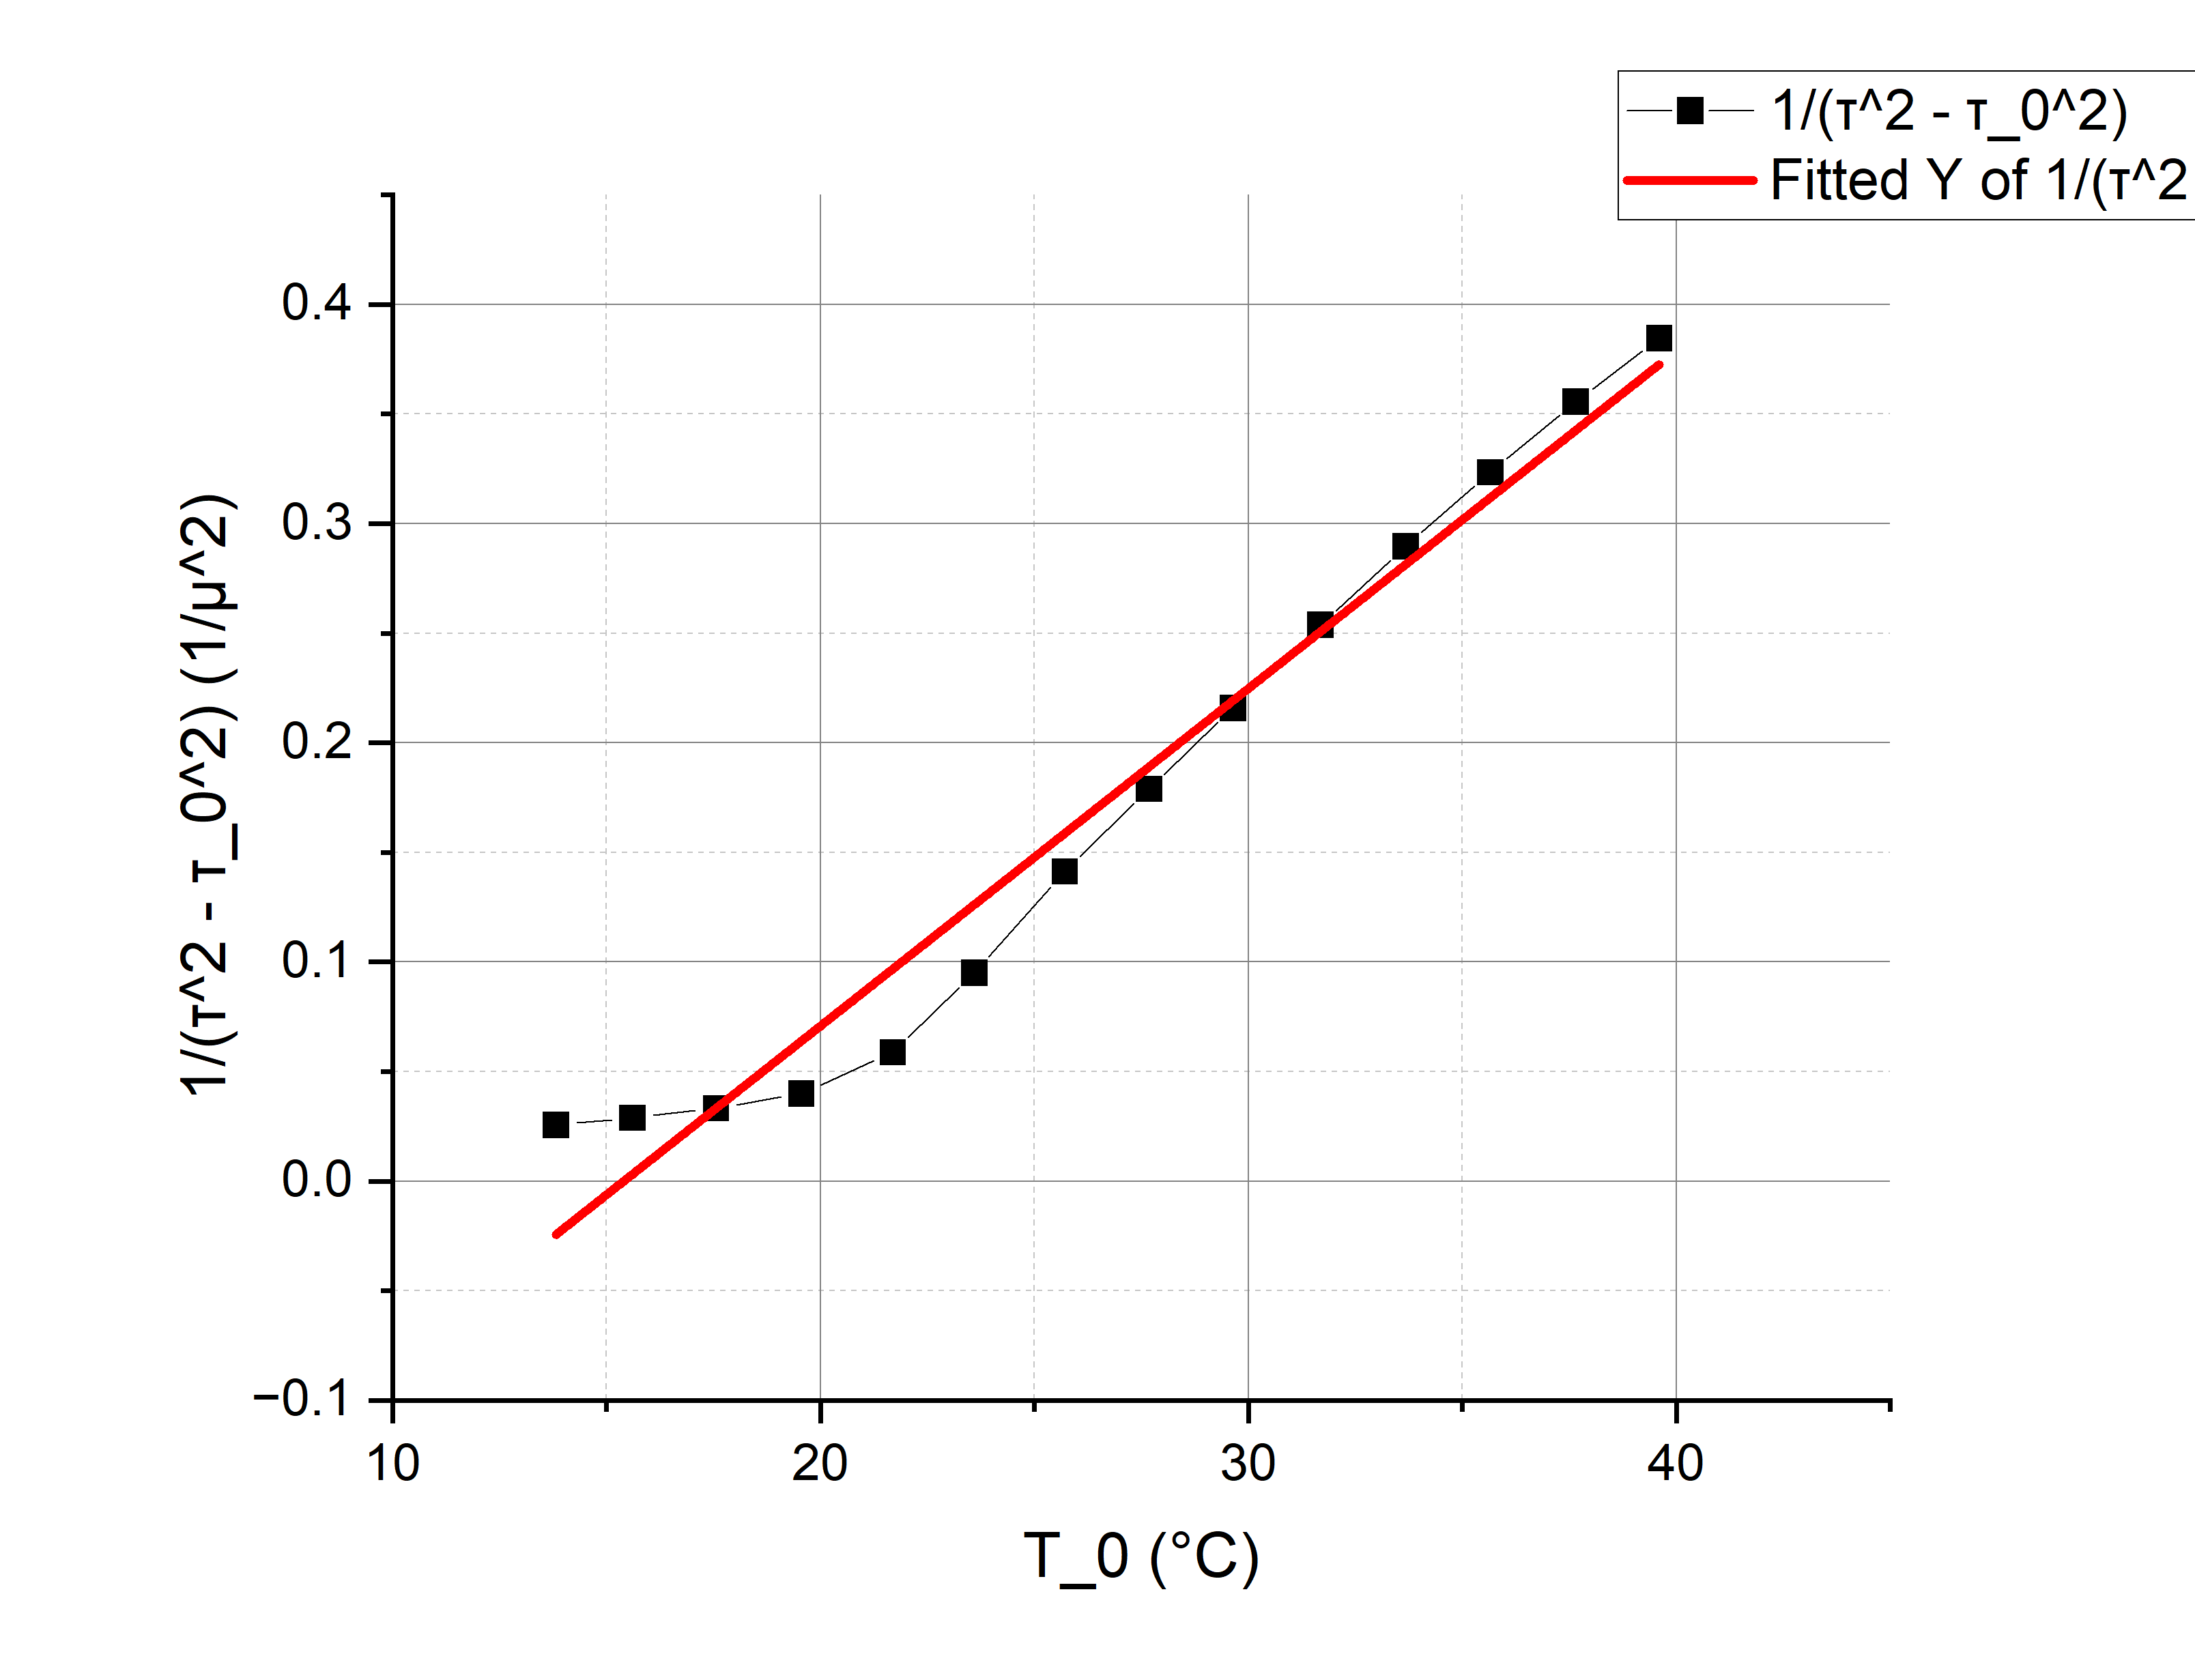
\includegraphics[scale=0.5]{Fig3.png}}
		\caption{ $1 / (\tau^2 - \tau_0^2)$ vs $T_0^{\circ} \mathrm{C}$ graph}
		\label{ris:ustanovka}
\end{figure} 
\begin{figure}
		\center{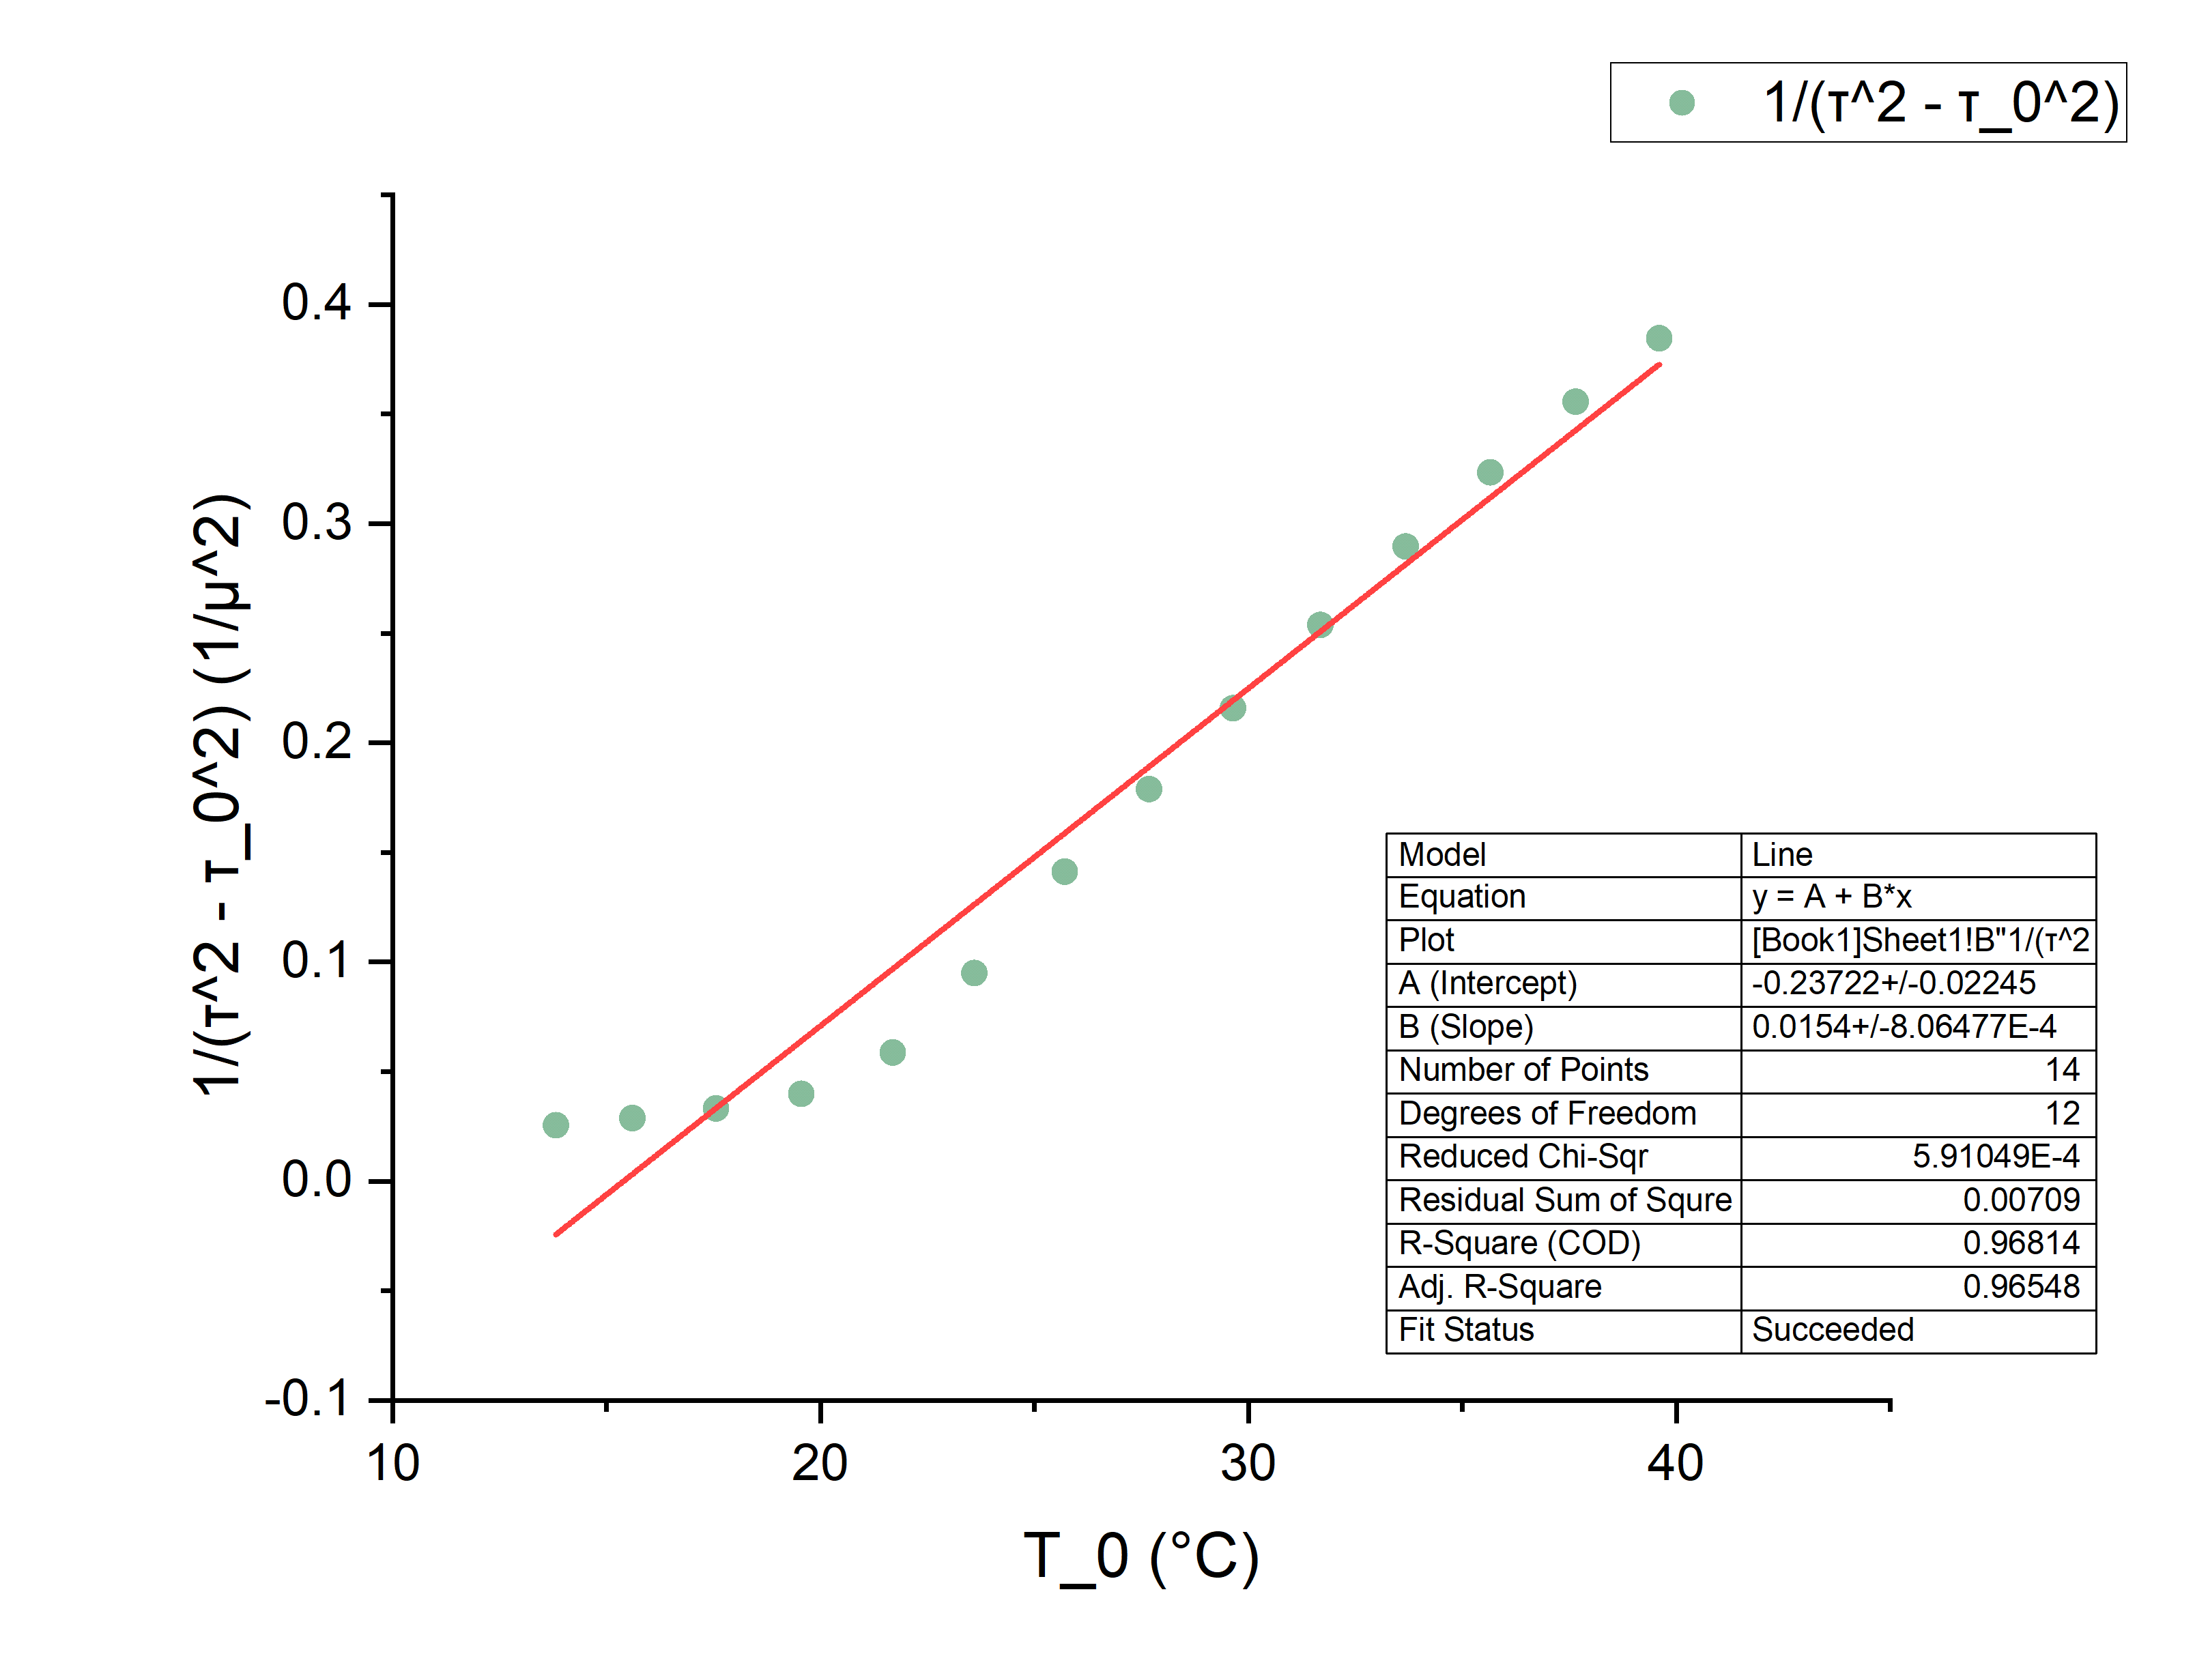
\includegraphics[scale=0.5]{Fig4.png}}
		\caption{$1 / (\tau^2 - \tau_0^2)$ vs $T_0^{\circ} \mathrm{C}$ graph with best fit line parameters}
		\label{ris:ustanovka}
\end{figure} 

\newpage
Now let's see the graph of $1 / (\tau^2 - \tau_0^2)$ vs $T_0^{\circ} \mathrm{C}$. From the best fit line's parameters we see that the desired Curie point $\Theta$, which is observed in the expected place for it (according to Wikipedia, $ \Theta = 19 \; ^\circ C$). Figure 3 shows that the graph turns into a straight line almost parallel to the abscissa axis, close to zero, also in the region of $19\; ^\circ C$.\\
\newline
According to the data of figure 4, we get a straight line
\begin{equation}
 \dfrac{1}{ \tau^2 - \tau_0^2} = 0.0154 \ T_o - 0.23722
\end{equation}

At 0 on the ordinate axis, the Curie temperature $ \Theta_p = \frac{a}{b} = \dfrac{0.23722}{0.0154} \approx 15.40 \; ^\circ C$. The error of the obtained value:
\begin{equation}
\sigma_{\Theta_p} = \Theta_p \sqrt{(\dfrac{\sigma_a}{a})^2 + (\dfrac{\sigma_b}{b})^2} = 1.67 ^\circ C
\end{equation}
\section{Conclusion}
Based on the results of the work done, we calculated the Curie point for Gadolinium:
\begin{center}
	{\fbox{ $ \Theta_p = (15.40 \pm 1.67) \; ^\circ C$}} \\
\end{center} 
From Wikipedia, we found the exact Curie temperature of Gadolinium is $19^\circ C$. We see our measurement result is little bit lower than the exact value and the accuracy of our measurement is $81.05\%$. The possible reason for this error is a type of human error while taking the data during the experiment. We can reduce this error and make our measurement more accurate by taking data carefully.








\end{document}